% (The MIT License)
%
% Copyright (c) 2023-2024 Yegor Bugayenko
%
% Permission is hereby granted, free of charge, to any person obtaining a copy
% of this software and associated documentation files (the 'Software'), to deal
% in the Software without restriction, including without limitation the rights
% to use, copy, modify, merge, publish, distribute, sublicense, and/or sell
% copies of the Software, and to permit persons to whom the Software is
% furnished to do so, subject to the following conditions:
%
% The above copyright notice and this permission notice shall be included in all
% copies or substantial portions of the Software.
%
% THE SOFTWARE IS PROVIDED 'AS IS', WITHOUT WARRANTY OF ANY KIND, EXPRESS OR
% IMPLIED, INCLUDING BUT NOT LIMITED TO THE WARRANTIES OF MERCHANTABILITY,
% FITNESS FOR A PARTICULAR PURPOSE AND NONINFRINGEMENT. IN NO EVENT SHALL THE
% AUTHORS OR COPYRIGHT HOLDERS BE LIABLE FOR ANY CLAIM, DAMAGES OR OTHER
% LIABILITY, WHETHER IN AN ACTION OF CONTRACT, TORT OR OTHERWISE, ARISING FROM,
% OUT OF OR IN CONNECTION WITH THE SOFTWARE OR THE USE OR OTHER DEALINGS IN THE
% SOFTWARE.

\documentclass{article}
\usepackage{../sqm}
\newcommand*\thetitle{Function Points}
\begin{document}

\plush{\sqmTitlePage{17}{}}

\qte
  {capers-jones.jpg}
  {From the start of the software era in the 1950s until roughly 1970, software cost estimating was performed \ul{manually}, using simple \ul{rules of thumb} or local estimating algorithms developed through trial and error methods.}
  {jones2007}

\qte
  {fred-brooks.jpg}
  {Our techniques of estimating are \ul{poorly developed}. More seriously, they reflect an unvoiced assumption which is quite untrue, i.e., that \ul{all will go well}.}
  {brooks1995mythical}

\qte
  {lawrence-putnam.jpg}
  {\textbf{SLIM}: In general, the \ul{size} of the product in source \ul{statements} is \(S = C \times K^{1/3} \times t^{4/3}\), where \(C\) is a productivity constant, \(K\) is development effort, and \(t\) is time.}
  {putnam1978general}

\qte
  {barry-boehm.jpg}
  {\textbf{COCOMO}: We compute the \ul{estimated development effort} as the nominal development effort times the product of the effort multipliers for the 15 \ul{cost driver attributes}... A nominal development effort is estimated as a function of the product's size in delivered source \ul{instructions} in thousands (KDSI) and the project's development mode.}
  {boehm1984software}

\qte
  {allan-albrecht.jpg}
  {\textbf{FPA}: The general approach is to count the number of external user \ul{inputs}, \ul{inquiries}, \ul{outputs}, and master \ul{files} delivered by the development project. These factors are outward manifestations of any application. They cover all the functions in an application.}
  {albrecht1979measuring}

\pitch{\begin{multicols}{2}
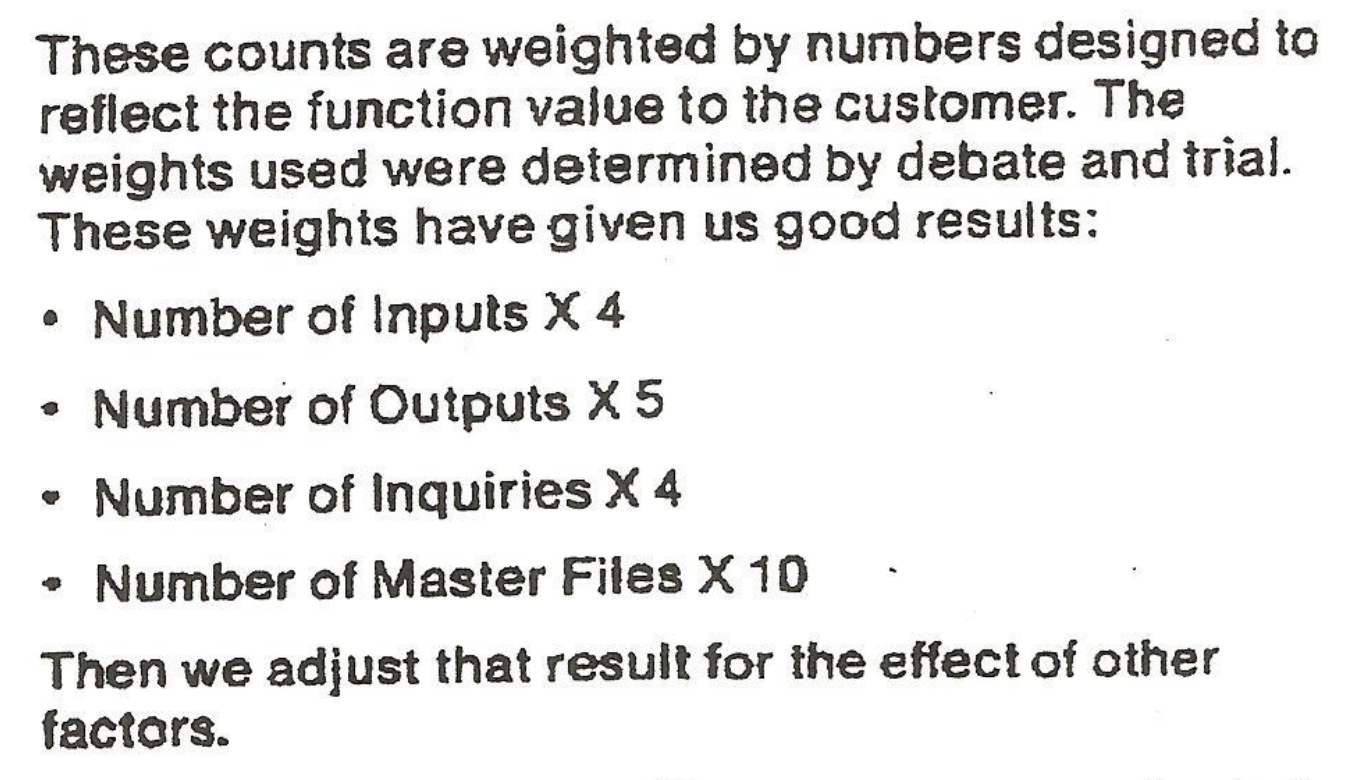
\includegraphics[width=\linewidth]{factors.png}
\par\columnbreak\par
``If the inputs, outputs, or files are extra complicated, we add 5\%. Complex internal processing can add another 5\%. On-line functions and performance are addressed in other questions. The maximum adjustment possible is 50\%, expressed as \(\pm\)25\% so that the weighted summation is the average complexity.''\par
{\scriptsize Source: \bibentry{albrecht1979measuring}\par}
\end{multicols}}

\pitch{\begin{multicols}{2}
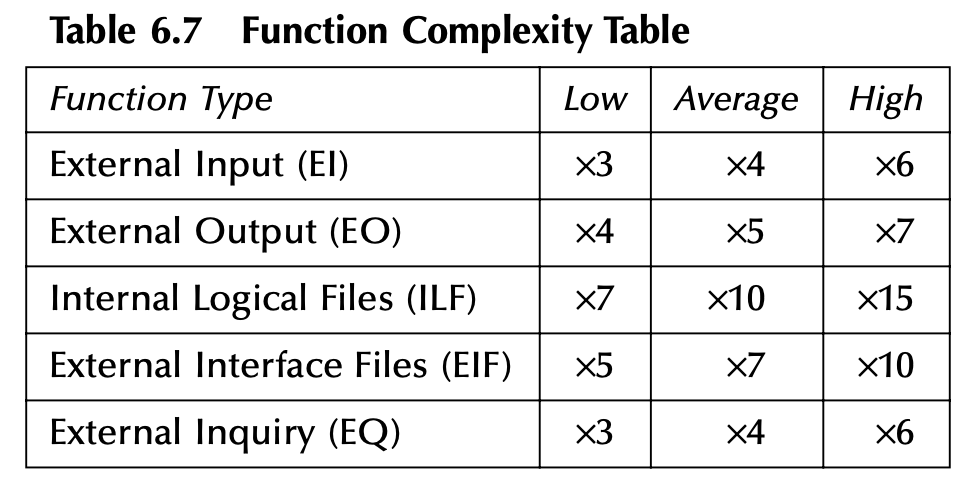
\includegraphics[width=\linewidth]{functions.png}
\par\columnbreak\par
``In order to find the adjusted function point (AFP) value, the UFP (the raw function count weighted by the appropriate complexity shown in the Table) is multiplied by the VAF.''\par
{\scriptsize Source: \bibentry{galorath2006software}\par}
\end{multicols}}

\qte
  {peter-chen.jpg}
  {The entity-relationship (ER) model adopts the more natural view that the real world consists of \ul{entities} and \ul{relationships}. It incorporates some of the important semantic information about the real world.}
  {chen1976entity}

\pitch{
\pptPic{.95}{er-diagram.png}
\par
{\scriptsize Source: \bibentry{chen1976entity}\par}}

\qte
  {tom-demarco.jpg}
  {The Data Flow Diagram shows flow of \ul{data}, not of \ul{control}. This is the difference between Data Flow Diagrams and flowcharts. The Data Flow Diagram portrays a situation from the point of view of the data, while a flowchart portrays it from the point of view of those who act upon the data.}
  {demarco1978}

\pitch{
\pptPic{.75}{dfd.png}
\par
{\scriptsize Source: \bibentry{demarco1978}\par}}

\qte
  {sloc-vs-fps.png}
  {At least for the applications analyzed, both the development work-hours and application size in ``SLOC'' are \ul{strong functions} of ``function points'' and ``input/output data item count.'' Further, it appears that basing applications development effort estimates on the amount of function to be provided by an application rather than an estimate of ``SLOC'' may be \ul{superior}.}
  {albrecht1983software}

\qte
  {book-of-charles-symons.jpg}
  {The major difference is that \textbf{Mk II FPA}, with its \ul{finer granularity}, is a continuous measure whereas IFPUG limits component size once a threshold is reached.}
  {symons1991software}

\pitch{
\pptPic{.95}{mk-ii.png}
\par
{\scriptsize Source: \bibentry{symons1991software}\par}}

\qte
  {daniel-galorath.jpg}
  {\textbf{SEER-SEM} is based on the concept that if a user can describe the \ul{essential characteristics} of a project and range of size, SEER-SEM can provide estimates of schedules, efforts, staffing, risks, uncertainties, and defects, characterizing each as a most likely \ul{estimate} or a risk estimate.}
  {galorath2006software}

\pitch{\begin{multicols}{2}
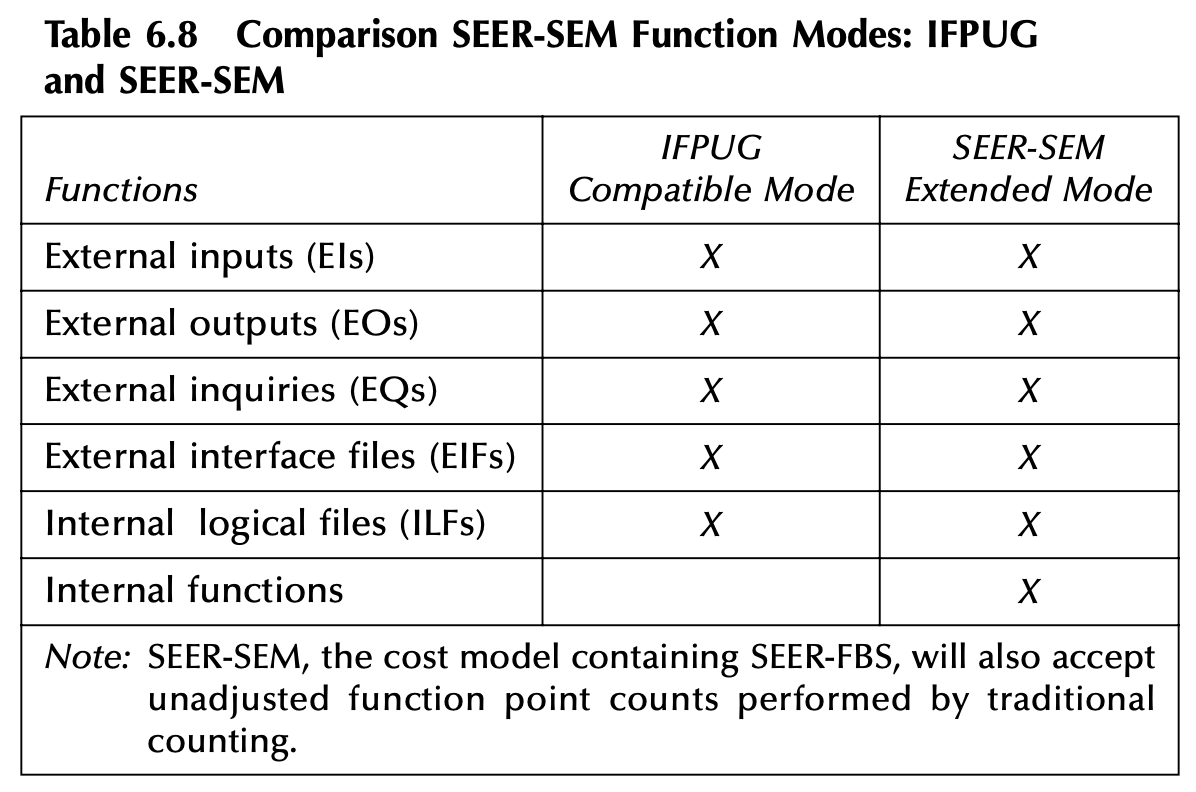
\includegraphics[width=\linewidth]{seer-fbs.png}
\par\columnbreak\par
``SEER-FBS (``function-based sizing''), introduced in 1992, is consistent with IFPUG counting rules, but adds a sixth category (\ul{internal functions}) that allows users to account for highly algorithmic processes of systems such as real-time and embedded-type systems.''\par
{\scriptsize Source: \bibentry{galorath2006software}\par}
\end{multicols}}

\qte
  {cocomo-2.jpg}
  {\textbf{COCOMO-II}: Success in all types of organization depends increasingly on the development of customized software solutions, yet more than half of software projects now in the works will \ul{exceed} both their \ul{schedules} and their \ul{budgets} by more than 50\%.}
  {boehm2000}

\pitch{\begin{multicols}{2}
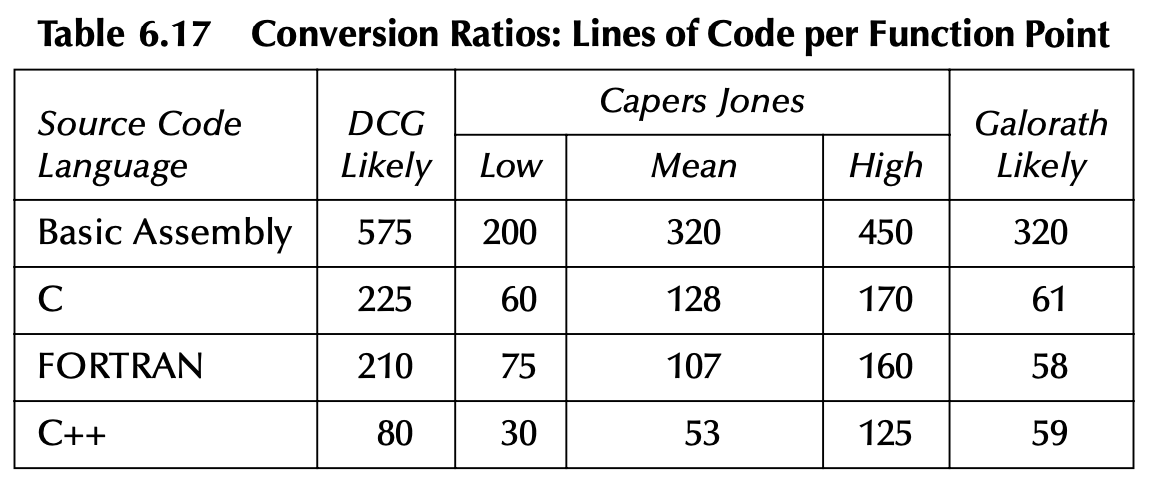
\includegraphics[width=\linewidth]{loc-per-fp.png}
\par\columnbreak\par
``\ul{Backfiring} is converting lines of code to function points by dividing the line count by a \ul{conversion ratio}. The author does not recommend backfiring as an approach to generating function points.''\par
{\scriptsize Source: \bibentry{galorath2006software}\par}
\end{multicols}}

\qte
  {capers-jones.jpg}
  {The reliability of function point analysis is good enough to allow function points to serve as the \ul{basis} for contracts, for carrying out scholarly research, for cost estimating, and for creating reliable benchmarks. In fact, function points are now \ul{used} for more business purposes than any other metric in the history of software.}
  {iso20926foreword}

\plush{
\pptBanner{IFPUG Procedure}
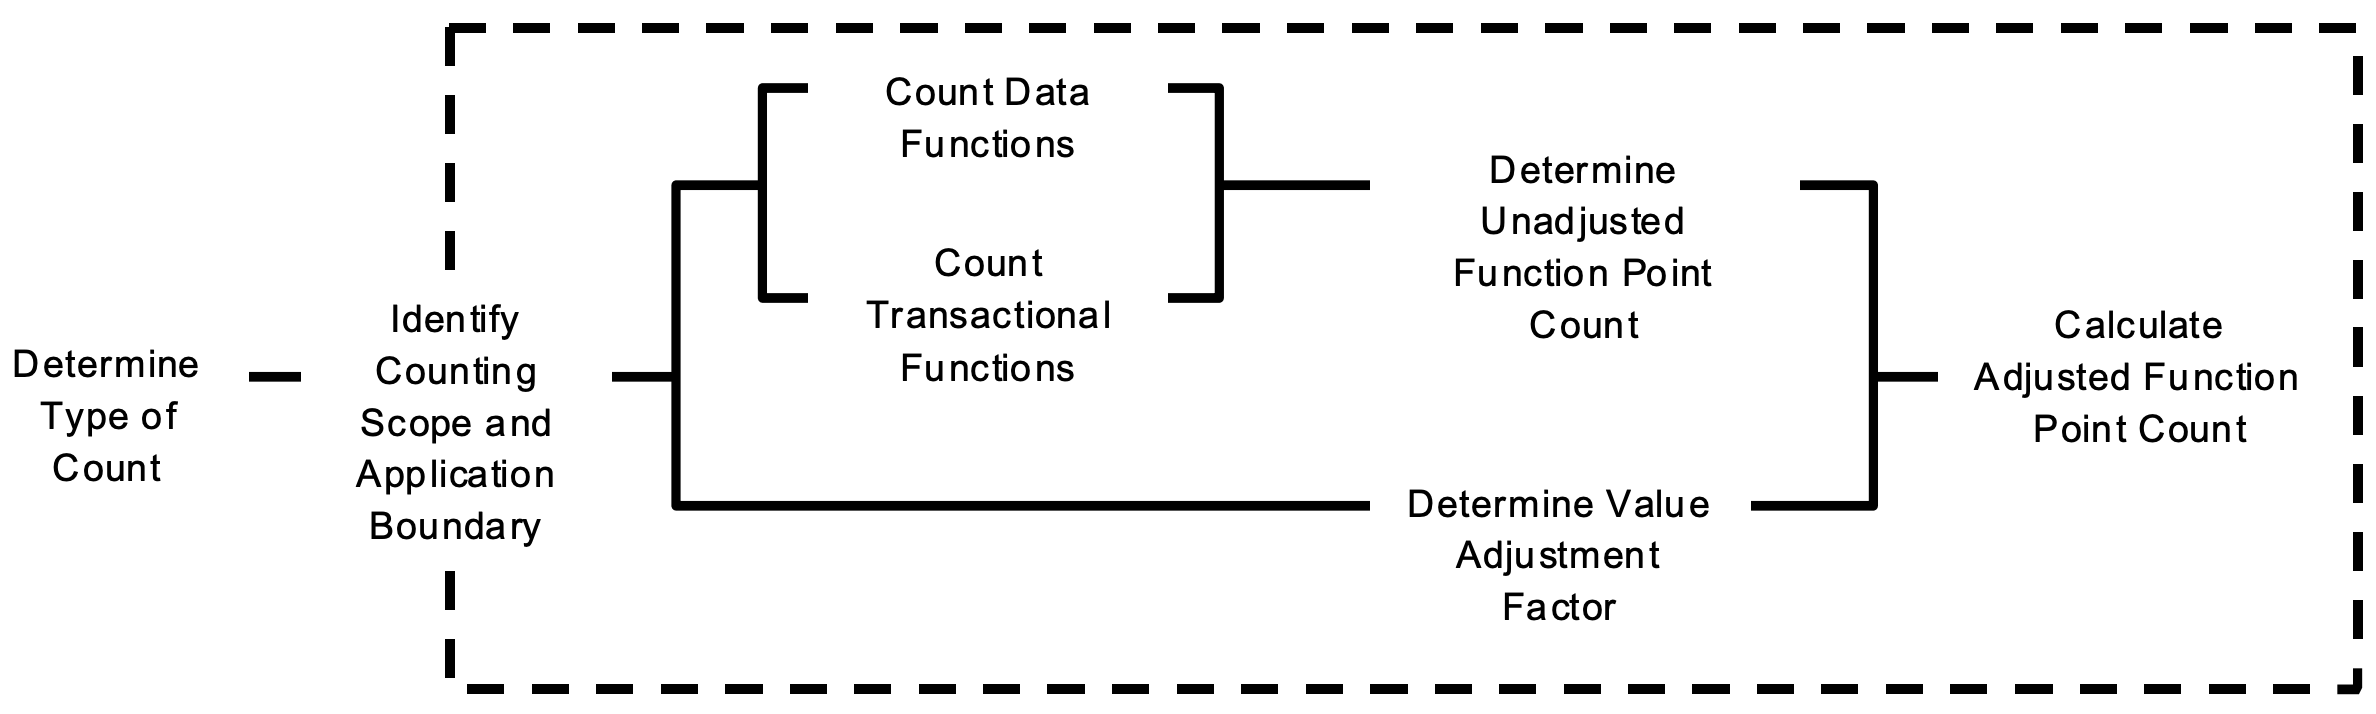
\includegraphics[width=\linewidth]{ifpug-procedure.png}
\par
{\scriptsize Source: \bibentry{iso20926}\par}}

\pitch{\begin{multicols}{2}
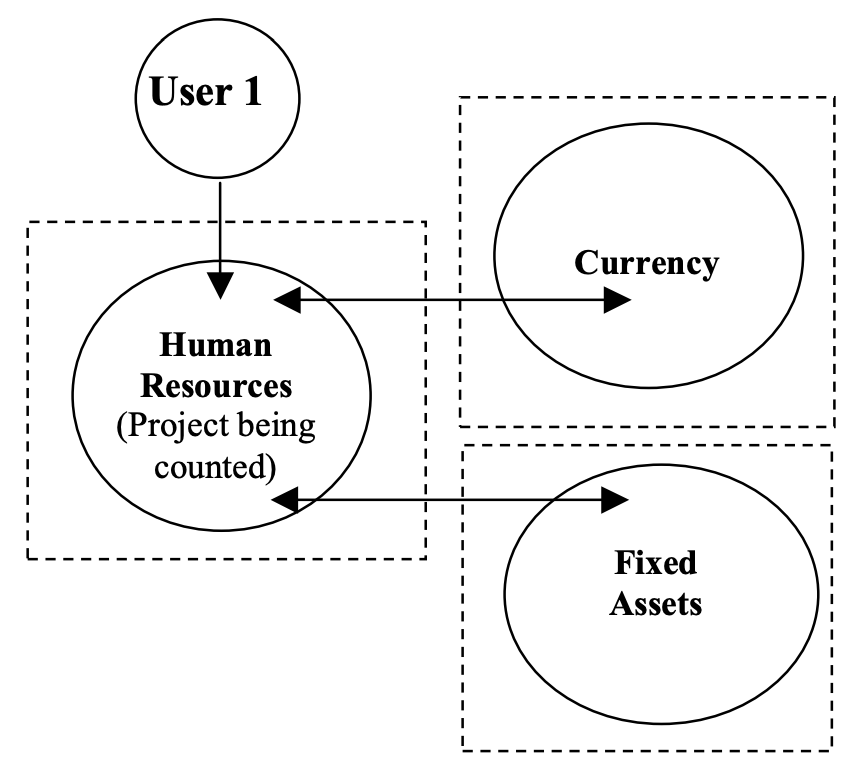
\includegraphics[width=\linewidth]{boundary.png}
\par\columnbreak\par
``The application \ul{boundary} indicates the border between the \ul{software} being measured and the \ul{user}.''\par
{\scriptsize Source: \bibentry{iso20926}\par}
\end{multicols}}

\pitch{\begin{multicols}{2}
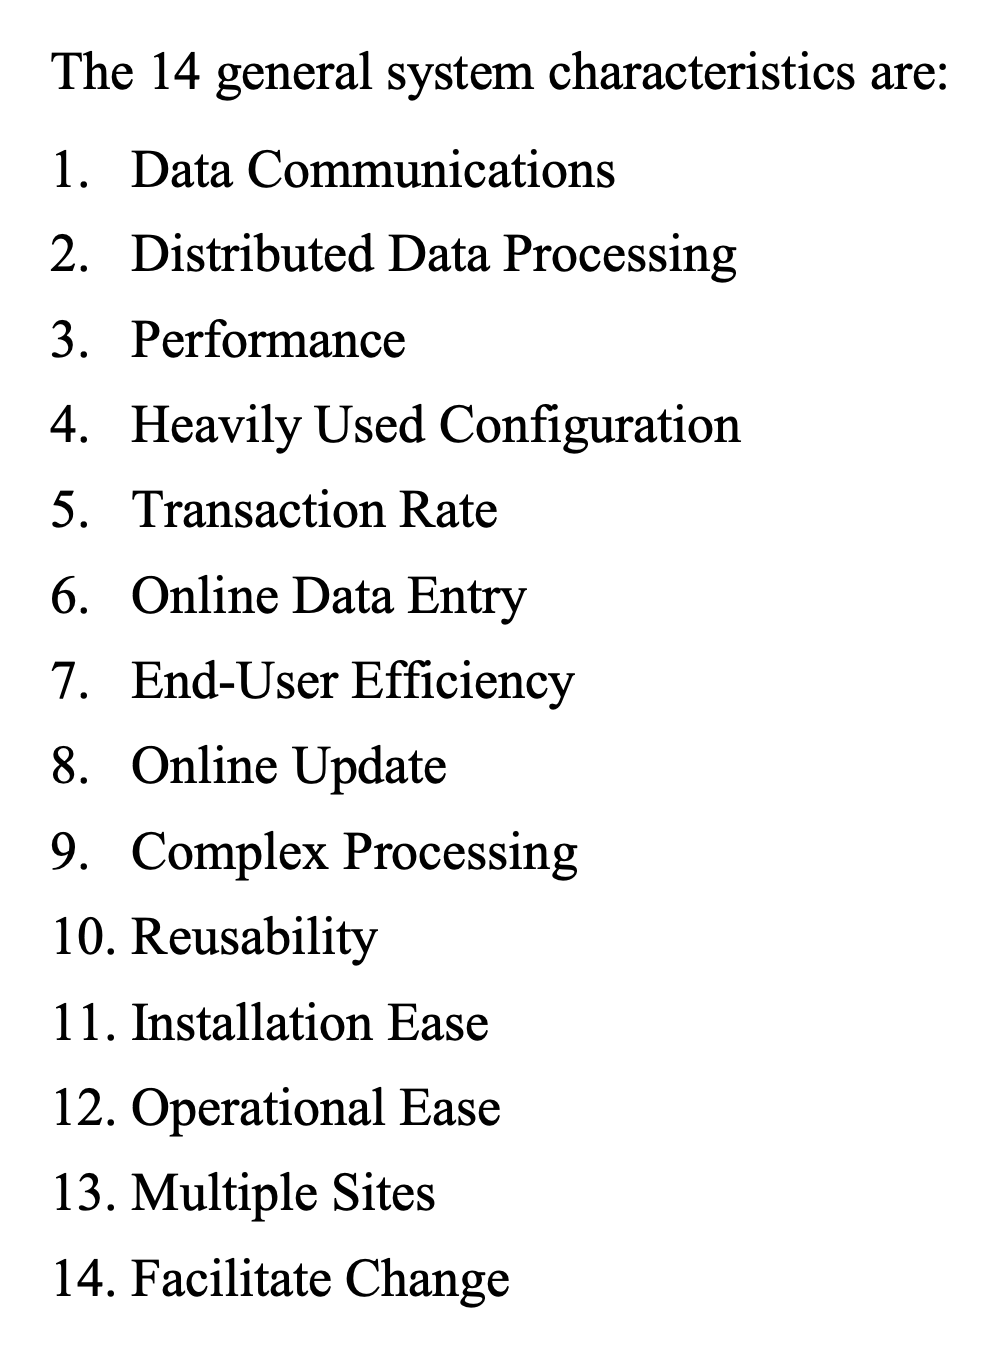
\includegraphics[width=.7\linewidth]{characteristics.png}
\par\columnbreak\par
``The 14 general system \ul{characteristics} are summarized into the \ul{value adjustment factor} (VAF). When applied, the value adjustment factor adjusts the \ul{unadjusted function point count} \(\pm\)35 percent to produce the \ul{adjusted function point count}.''\par
{\scriptsize Source: \bibentry{iso20926}\par}
\end{multicols}}

\pitch{\begin{multicols}{2}
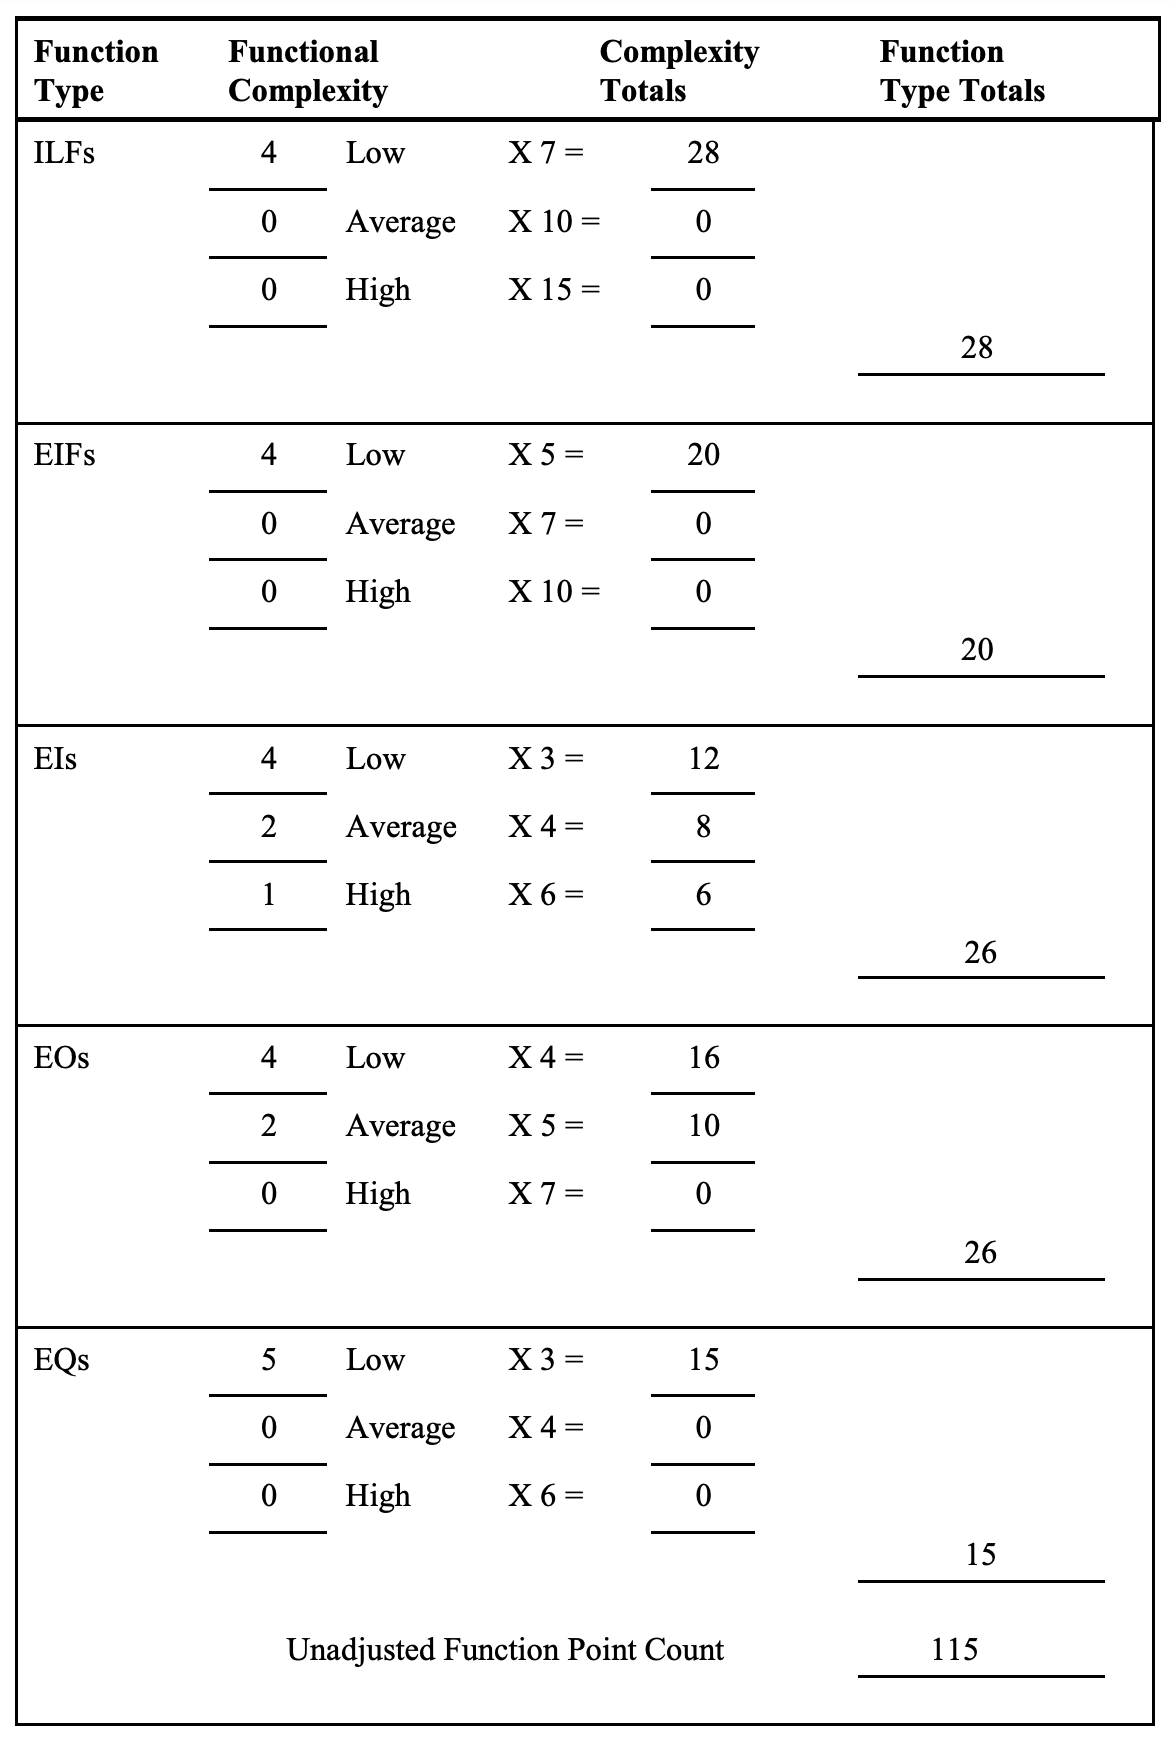
\includegraphics[width=.65\linewidth]{ufpc-example.png}
\par\columnbreak\par
``The formula calculates the \ul{development project function points}: \texttt{DFP = (UFP + CFP) * VAF}.
Where
UFP is the unadjusted function points for the functions that will be available after installation,
and
CFP is the unadjusted function points added by the conversion unadjusted function point count.''\par
{\scriptsize Source: \bibentry{iso20926}\par}
\end{multicols}}

\qte
  {roger-pressman.jpg}
  {The function point metric, like LOC, is relatively \ul{controversial}... Opponents claim that the method requires some `sleight of hand' in that computation is based on \ul{subjective}, rather than \ul{objective}, data.}
  {pressman2005software}

\pitch{\pptBanner{Function Point Standards}
\begin{itemize}\setlength\itemsep{0pt}
\item Mark-II --- ISO/IEC 20968:2002
\item IFPUG --- ISO/IEC 20926:2009
\item FiSMA --- ISO/IEC 29881:2010
\item COSMIC --- ISO/IEC 19761:2011
\item Nesma --- ISO/IEC 24570:2018
\item OMG --- ISO/IEC 19515:2019
\end{itemize}}

\pitch{\pptBanner{Some Other Function Points}
\begin{itemize}\setlength\itemsep{0pt}
\item Early and easy function points
\item Engineering function points
\item Object-Oriented Function Points (OOFP)
\item Weighted Micro Function Points
\item Fuzzy Function Points
\end{itemize}}

\end{document}
